\subsection{Opgaver}

\begin{enumerate}
\item Løs ligningerne
\begin{align*}
8x+2=26,&& -3x-5=4,&&-6x+7=-29,&& 8x+11=5.
\end{align*}

\item Løs ligningerne
\begin{align*}
3x+7=-2x+2,&& 3(x-4)+2=2(x+1),&& -3x-4=-x+3.
\end{align*}

\item Løs ulighederne 
\begin{align*}
2x<4-5x,&& x-3>2-x,&& 2x-3\geq 2x,&& -2x\leq2(x-7).
\end{align*}

\item Betragt ligningen
\begin{align*}
ax+4=-x+b.
\end{align*}
Brug \href{https://www.geogebra.org/m/Q4Wh3Xrj}{Geogebra} til at visualisere alle værdier af $a$ og $b$ så at
\begin{enumerate}
\item Ligningen har præcis en løsning.
\item Ligningen har ingen løsning.
\item Ligningen har uendeligt mange løsninger.
\end{enumerate}

\item Løs ligningerne
\begin{align*}
 3(x-2)+2=3x-8,&& -(x+1)+2x=2(x-1)-x+1
\end{align*}

\item Løs ligningerne 
\begin{align*}
\frac{1}{x-2}=5,&& \frac{x^2+8}{x+2}=x+2,&& \frac{5}{x-1}=\frac{7}{x},&&  \frac{x^2+9-6x}{2x^2-6x}=1.
\end{align*}

\item Løs ligningerne
\begin{align*}
\frac{2}{3}\Big(x- \frac{5}{2}\Big)=\frac{3}{6},&& \frac{3}{8}(4x-2)=-\frac{1}{3}\Big(x-\frac{3}{4}\Big)
\end{align*}

\item Løs ligningerne
\begin{align*}
\sqrt{2}x+4=8,&& \pi(x-1)=\sqrt{2}x+3,&& \sqrt{2}(2\sqrt{2}x-\sqrt{8})=2x+1.
\end{align*}

\item Angiv hvilken figur i planen afgrænses af følgende uligheder, for polygoner angiv hjørnernes koordinater, for cirkelskiver angiv radius og centrumskoordinater.
\begin{enumerate}
	\item $ 0\leq x\leq 2, 0\leq y\leq 2 $
	\item $ x^2+y^2\leq 4 $
	\item $ 0\leq x\leq 2, 0 \leq y\leq 2x+2 $.
\end{enumerate}


\item Opstil uligheder der beskriver de grå områder der ses i Figur~\ref{fig:ligninger1}
\begin{figure}
\centering
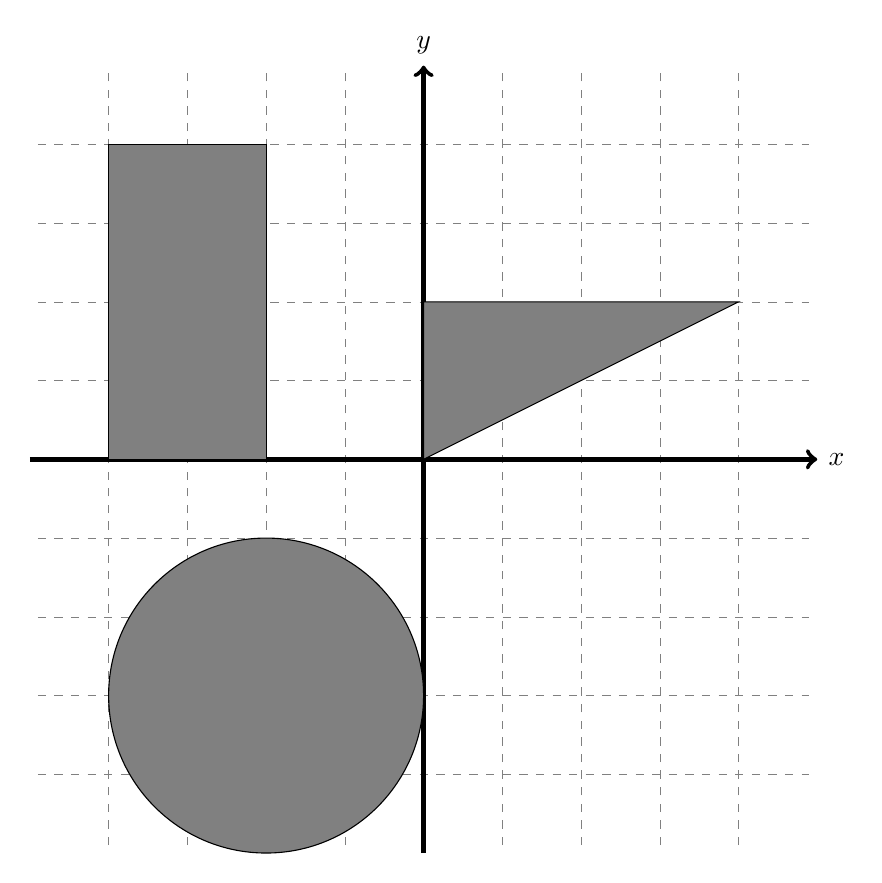
\begin{tikzpicture}
\draw[help lines, color=gray, dashed] (-4.9,-4.9) grid (4.9,4.9);
\draw[->,ultra thick] (-5,0)--(5,0) node[right]{$x$};
\draw[->,ultra thick] (0,-5)--(0,5) node[above]{$y$};

\draw[fill=gray] (-2,-3) circle (2);
\draw[fill=gray] (0,0)--(0,2)--(4,2)--cycle;
\draw[fill=gray] (-4,0)--(-2,0)--(-2,4)--(-4,4)--cycle;
\end{tikzpicture}
\caption{Find uligheder der beskriver de grå områder.}
\label{fig:ligninger1}
\end{figure}

\item Vis at 
\begin{align*}
ab\leq \frac{a^2}{2}+\frac{b^2}{2}.
\end{align*}
(Hint: Betragt $(a-b)^2$.)
Find derefter tal $a, b, c, d$ så
\begin{align*}
ab= \frac{a^2}{2}+\frac{b^2}{2},\quad \textup{og} \quad cd<\frac{c^2}{2}+\frac{d^2}{2}.
\end{align*}

\item Vis at
\begin{align*}
\sqrt{a+b}\leq \sqrt{a}+\sqrt{b},
\end{align*}
for $a,b\geq 0$.
(Hint: betragt $ (\sqrt{a}+\sqrt{b})^2 $). Find derefter $a,b,c,d\geq 0$ således at
\begin{align*}
\sqrt{a+b}=\sqrt{a}+\sqrt{b},\quad \textup{og}\quad \sqrt{c+d}<\sqrt{c}+\sqrt{d}.
\end{align*}

\end{enumerate}